% !TeX root = ../praktikum.tex
% !TeX encoding = UTF-8
% !Tex spellcheck = de_DE


Analog zur Auswertung der Gleichstrommessung wurde auch für die aufgenommenen Messdaten der Wechselstrommessung, abgebildet in Graphik \ref{fig:full_range_ac} und \ref{fig:2T_range_ac}, die Dichte der Ladungsträger im 2DEG, sowie deren Beweglichkeit bestimmt.

\subsubsection{Näherung über die Hall-Spannung}
\label{ch:naeherung_hall2}

Wie in der Auswertung der Gleichstrommessung wurden auch hier die beiden physikalischen Größen zunächst über die Steigung des klassischen Teils der Hallspannung zwischen \unit[-1]{T} und \unit[1]{T} bestimmt.
\begin{equation}
	\d{U_{Hall}}{B} = ( 18,7604 \pm 0,0030 ) \cdot 10^{-4} ~ \unitfrac{m^2}{s}
\end{equation} %1,87604E-03	3,04635E-07
Dabei wurde von den gemessene Strom der Mittelwert für diesen Bereich ermittelt: $I=\unit[0,978]{\mu A}$. Analog zur Auswertung der Gleichstrommessdaten ergaben sich hier für die gesuchten Größen folgende Werte: 
\begin{align}
n_s=  ( 7,15761 \pm 0,00015) \cdot 10^{15} ~ \unitfrac{1}{m^2}\\ %7,15761E+15	1,45547E+12
\mu= (26,19592\pm 0,00533) \cdot 10^6 ~ \unitfrac{m^2}{Vs} %2,61959E+07	5,32791E+03
\end{align}


\subsubsection{Näherung über die Shubnikov-de Haas-Oszillation}
\label{ch:naeherung_ac}

Ebenfalls analog zur Gleichstrommessung wurden die gesuchten physikalischen Größen alternativ über die Shubnikov-de Haas-Oszillation berechnet. Dies ist in Abbildung~\ref{fig:ac_sdho_ausw} zu sehen. 
Es ergibt sich eine Steigung der Geraden von $b=(28,9081 \pm 0,0358)\unit{T}$ und daraus analog zum vorherigen Versuchsteil die physikalischen Größen: 
\begin{align}
n_s= (6,9899 \pm 0,0087)\cdot 10^{11} \cdot \unitfrac{1}{m^2} \\ % 6,98995E+15	8,65203E+12
\mu= (26,82425 \pm 0,03325)\cdot 10^6 ~ \unitfrac{m^2}{Vs} %2,68242E+07	3,32437E+04
\end{align} 
   
\begin{figure}[h]
	\centering
	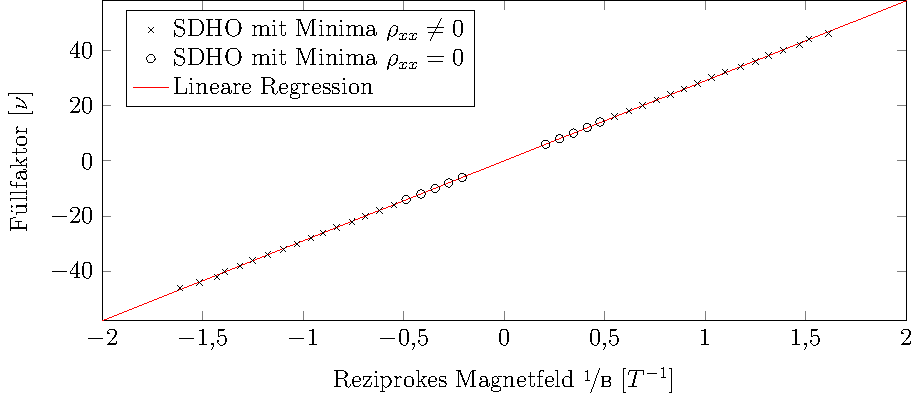
\includegraphics{graphs/ac/auswertung.pdf}
	\caption[Lineare Regression Wechselstrommessung]{
		Lineare Regression über den Füllfaktor der QHE-Plateaus der Wechselstrommessung aufgetragen gegen das Reziproke Magnetfeld.
	}
	\label{fig:ac_sdho_ausw}
\end{figure}

\begin{equation}
\nu= A\cdot \nicefrac{1}{B}=(28.908\pm 0.035)T \cdot \nicefrac{1}{B}
\end{equation}

Es wurde ein Offset von $\nu=4$ benutzt.